\documentclass[conference]{IEEEtran}
\IEEEoverridecommandlockouts

\usepackage{cite}
\usepackage{amsmath,amssymb,amsfonts}
\usepackage{graphicx}
\graphicspath{{../figures/}{./}}  % in the repo, figures/ sits next to report/; otherwise use this folder
\usepackage{textcomp}
\usepackage{xcolor}
\usepackage{booktabs}   % \toprule, \midrule, \cmi
\usepackage{xurl}       % \url, breakable anywhere
\usepackage[hidelinks]{hyperref}

% Wider text block: side margins reduced by 12pt each (columns 252pt -> 264pt)
\addtolength{\textwidth}{24pt}
\addtolength{\oddsidemargin}{-12pt}
\addtolength{\evensidemargin}{-12pt}
\setlength{\columnwidth}{\dimexpr(\textwidth-\columnsep)/2\relax}

% Lets the authors wrap onto a second row (2 x 2 grid)
\makeatletter
\newcommand{\linebreakand}{%
  \end{@IEEEauthorhalign}
  \hfill\mbox{}\par
  \mbox{}\hfill\begin{@IEEEauthorhalign}
}
\makeatother

\begin{document}

\title{Siloed or Universal? An Empirical Study of Cross-Language Agent Skill Reuse in GitSkills}

\author{\IEEEauthorblockN{Tristan Lachance (2141919)}
\and
\IEEEauthorblockN{Laurel Tremblay (2141998)}
\linebreakand
\IEEEauthorblockN{Sebastian Espin Ontiveros (2132717)}
\and
\IEEEauthorblockN{Jonathan Roy-Ascanio (2152552)}
}

\maketitle

% All the body text (abstract -> conclusion) lives in report.tex
% report.tex -- body of the paper, included by main.tex with % report.tex -- body of the paper, included by main.tex with % report.tex -- body of the paper, included by main.tex with \input{report}.
% No preamble here: no \documentclass, \usepackage or \begin{document}.

\begin{abstract}
Agent skills are \texttt{SKILL.md} files written in natural language, so unlike code libraries, which are tied to one language's package ecosystem, they could in principle be reused in any project. Using the GitSkills dataset (3.8 million \texttt{SKILL.md} files in 282,200 GitHub repositories), we find that exact copies of skills often cross programming languages, but far less than in a baseline where language plays no role (57.6\% vs.\ 87.0\%). Those cross-language ties mostly follow shared runtimes and platforms. Since skills that cross languages and skills that do not look almost the same, agent skills seem to reproduce the language silos of package ecosystems for social rather than technical reasons.
\end{abstract}

\section{Introduction}
Traditional software dependencies are tied to a specific programming language and its package ecosystem~\cite{decan2019empirical}. JavaScript libraries are distributed through npm, for example, while Python libraries use PyPI, with each language maintaining its own independent ecosystem. Because these dependencies rely on compilers, specific runtimes, and build toolchains, reuse across language boundaries normally requires wrappers, bindings, or some level of reimplementation. AI coding agents introduce a different possibility through natural-language artifacts, most notably \texttt{SKILL.md} files, which encode workflows, conventions, and recurring developer instructions. Unlike executable code libraries, these artifacts are not bound to a package manager and could therefore be reused across repositories with completely different technology stacks without extra manual effort.

Writing a skill in natural language does not automatically make it portable, however. In practice, a skill can still include language-specific scripts, rely on tools tied to a particular stack, or simply circulate within a single language community, even though nothing in the format itself forces skills to stay siloed. As a result, it remains an open question whether developers are building a unified, language-agnostic skill ecosystem or recreating the same fragmented silos seen in traditional software dependencies.

In this paper, we empirically investigate whether agent skills spread across programming language boundaries using the July 2026 GitSkills dataset~\cite{destefanis2027gitskills}. The dataset collects 3,797,117 \texttt{SKILL.md} files (1,877,981 distinct) across 282,200 public GitHub repositories, linking exact copies by content hash and pairing them with file contents and repository metadata, including each repository's primary programming language. Our goal is to determine whether verbatim skill copying crosses primary programming languages at rates consistent with a language-agnostic ecosystem, and to identify the structural and functional characteristics that distinguish skills that are adopted across multiple language projects from those that are confined to a single language.

Our results actually indicate that verbatim skill copying is only partially independent of programming language. Of the 67,061 skills copied by at least two distinct eligible owners, 57.6\% are adopted across more than one language, compared to 87.0\% in the language-agnostic ecosystem simulated by our baseline. Cross-language adoption is therefore common, yet substantially less frequent than it would be in a language-agnostic ecosystem, pointing to persistent language siloing. Among skills copied by the same number of owners, those adopted across three or more languages also differ from single-language skills, as they are less likely to contain code or scripts and are more frequently associated with language-independent topics such as planning, task management, and UI design. Still, these differences are limited in magnitude, suggesting that a skill's internal structure and topic only explain part of the language concentration we observe.

\section{Background and Related Work}

\subsection{Background}

An agent skill is a folder that contains a \texttt{SKILL.md} file with some YAML front matter (a name and its description) and a Markdown body of natural-language instructions along with optional scripts or some additional reference files~\cite{agentskills_spec,destefanis2027gitskills}. Introduced by Anthropic in October 2025 as an open specification, the format relies on runtime selection (using a probabilistic approach). More specifically, an AI coding agent reads all available skill descriptions added by the agent user and decides at runtime whether to load and use a skill for a given task or not given the current context~\cite{destefanis2027gitskills}. Since those skills do not have a central package manager, developers reuse them mainly by copying folders across repositories no matter the main technology stack of the project~\cite{destefanis2027gitskills}. To identify each repository's technology stack, GitHub actually uses \emph{Linguist}, which is a library that inspects repository files to assign it a primary language in its metadata and classify it as programming, markup, data, or prose. This information that is made available in the GitSkills dataset is fundamental to our research here.

Our analysis relies on four standard statistical and text-mining methods:
\begin{itemize}
    \item \textbf{Permutation testing:} Builds a chance baseline (null distribution) by repeatedly shuffling labels at random, testing how far an observed result departs from chance without parametric assumptions.
    \item \textbf{TF-IDF and NMF:} Term Frequency-Inverse Document Frequency (TF-IDF) converts text into vectors that weight terms frequent in a document but rare across the corpus; Non-negative Matrix Factorization (NMF) decomposes that matrix into interpretable topics.
    \item \textbf{Mann-Whitney U and Cliff's delta:} The Mann-Whitney U test compares two independent groups without assuming normality, while Cliff's delta measures the effect size in $[-1, 1]$ by quantifying how often values in one group exceed those in the other.
    \item \textbf{Chi-square and Cram\'er's V:} Pearson's chi-square test checks whether two categorical variables are associated, and Cram\'er's V scales the strength of that association to $[0, 1]$.
\end{itemize}


\subsection{Related Work}

Before AI coding agents became widespread, empirical work on software reuse focused mainly on artifacts that are directly tied to specific language ecosystems. Studies of package managers showed how dependency networks grow inside separate, language-bound registries such as npm, PyPI, and RubyGems~\cite{decan2019empirical}. Those silos are not only technical as comparing 18 open-source ecosystems, Bogart et al.~\cite{bogart2021breaking} actually showed that language communities also tend to build distinct norms and maintenance practices around their dependencies. Even outside package managers, informal copying reflects ecosystem boundaries. Lopes et al.~\cite{lopes2017dejavu} analyzed 4.5 million GitHub projects and found that 70\% of files are duplicates, with duplication rates varying widely by language (from 94\% in JavaScript to 40\% in Java).

With the arrival of coding agents, reuse studies have expanded to natural-language artifacts such as \texttt{SKILL.md} files among many new techniques for defining reusable artifacts, which are no longer bound to a single runtime. Early work shows that direct copying is still how most reuse happens. More precisely, in GitSkills dataset studied here, 50.5\% of public \texttt{SKILL.md} files are verbatim copies~\cite{destefanis2027gitskills}, and Gao et al.~\cite{gao2026registry} found that skills pulled from community registries into repositories are mostly one-time copies, with later edits focusing on project-specific bindings. At the artifact level, Zhang et al.~\cite{zhang2026keeps} audited 138K \texttt{SKILL.md} files and highlighted that specification and routing-metadata defects frequently limit reuse.

Prior work therefore establishes two things: traditional code reuse was shaped by both technical and community silos, and agent skills are widely copied yet often tied to local project setups. Still, none of these studies test whether natural-language skills actually cross programming-language boundaries or remain concentrated within single-language ecosystems, which is the gap we address here.

\section{Methodology}\label{sec:methodology}

\subsection{Research Questions}
In this study, we address two research questions:
\begin{description}[\IEEEsetlabelwidth{RQ2:}]
    \item[RQ1:] \textit{Ecosystem Silos vs. Universal Flow.} To what extent does the verbatim copying of agent skills bypass traditional programming language boundaries?
    \item[RQ2:] \textit{Anatomy of a Universal Skill.} What structural and functional characteristics distinguish skills adopted across many diverse primary languages from strictly siloed skills?
\end{description}

\subsection{Data Collection and Cleaning}
We use the July 2026 release of the GitSkills dataset~\cite{destefanis2027gitskills}, accessed via its official Hugging Face Parquet mirror (archived on Zenodo, DOI: 10.5281/zenodo.21875637). From it, we extract the \texttt{artifacts} table (3,797,117 \texttt{SKILL.md} files across 1,877,981 unique content hashes) and the \texttt{repos} table (282,200 repositories), keeping file hashes, representative skill contents, and repository metadata.

We clean the data in three stages. First, we filter for repositories whose primary language actually reflects project adoption. Using GitHub Linguist v9.6.0 (the release current at mining time), we keep only repositories with a programming language as their primary language (230,558), excluding markup, data, prose, and undetected languages. We also drop forks (3 repositories) and aggregators holding more than 100 distinct skills (2,829 repositories, just 1.0\% of repositories, yet 54.3\% of all \texttt{SKILL.md} files), since registries, mirrors, and marketplaces do not represent real project use and would bias our insights. This leaves 228,037 eligible repositories.

Second, we identify exact copies using each file's Git blob hash (\texttt{file\_sha}) and store one adoption record per unique skill--repository pair (with \texttt{n\_paths} counting duplicate paths within the same repo). Dropping 1,647,626 single-owner skills leaves 230,355 copied skills (found under at least two distinct owners) and 1,382,321 adoption records overall. We pull structural metadata from each skill's deduplicated representative row, and restrict our language analysis to the 67,061 copied skills adopted by at least two distinct eligible owners. This structural metadata includes each skill's text length, whether its front matter is valid, and whether its folder contains scripts or reference files, as recorded by GitSkills (\texttt{has\_scripts}, \texttt{has\_references}); skills with missing values are excluded from the corresponding comparison.

Third, we extract two content features from each copied skill's representative file. For code blocks, we parse Markdown code fences (\texttt{\`{}\`{}\`{}}) and map their tags to programming languages using Linguist aliases and groups (e.g., mapping \texttt{ts} and \texttt{TSX} to TypeScript). For functional purpose, we combine each skill's \texttt{name} and \texttt{description}, vectorize the text with TF-IDF (removing English stop words, keeping alphabetic tokens of length $\ge 2$ with \texttt{min\_df} $= 20$ and \texttt{max\_df} $= 0.5$), and apply 12-topic NMF (\texttt{nndsvd} initialization, fixed seed). Each skill receives its top-weighted topic (named after its three top terms, which we use to interpret what the topic is about), or \texttt{none} when all topic weights are zero (e.g., non-English or missing text).

\subsection{Analysis and Statistical Methods}
\textbf{RQ1 (Cross-Language Reuse).} Across these skills, we aggregate adoptions at the owner level so that one user copying a skill across many repositories counts only once. Each owner is assigned the most frequent primary language among their eligible repositories holding that skill. We label a skill \emph{cross-language} if its adopting owners span multiple primary languages, and \emph{siloed} otherwise. To account for adoption scale, we group skills into four owner-count tiers: 2, 3--5, 6--20, and $>20$ owners.

Because TypeScript and Python dominate GitHub, some cross-language overlap happens by chance. To separate it from real cross-language flow, we run a 1,000-iteration permutation baseline (fixed seed): in each iteration, we shuffle the primary language labels across skill--owner rows and recompute the overall and per-tier crossing rates. Their mean is the expected rate in a language-agnostic ecosystem (grey bars in Fig.~\ref{fig:crossing}), and the share of shuffles at or below the observed rate gives one-sided $p$-values.

To see which languages actually share skills, we build a co-adoption matrix for the 12 largest languages. For each skill with $k_s$ eligible owners, every pair of distinct owners contributes a language pair weighted by $1/(k_s - 1)$ so popular skills do not dominate. We then divide observed counts by the counts expected under random owner pairing, i.e., in a language-agnostic ecosystem ($>1$ means more sharing than in such an ecosystem).

\textbf{RQ2 (Universal vs. Siloed Skills).} Focusing on skills with at least three eligible owners, we compare \emph{universal skills} ($\ge 3$ primary languages; 14,186 skills) against \emph{siloed skills} (all owners in one language, as in RQ1; 9,104 skills), leaving out two-language skills to keep a clear contrast between the groups. Because popular skills naturally have more chances to span multiple languages, we match both groups on exact owner count by randomly subsampling to the smaller group's size at each count, leaving 6,678 matched pairs (5.1 owners on average).

We compare the matched groups across five structural features (body length, valid YAML front matter, bundled reference files, bundled scripts, and programming-language code blocks) using two-sided Mann--Whitney $U$ tests, Cliff's $\delta$ for effect size, and Bonferroni correction across the five tests, and we also break down code-block shares by individual language. We also test whether topic distributions (the 12 NMF topics plus \texttt{none}) differ between universal and siloed skills using a chi-square test and Cram\'er's $V$.

\subsection{Replication Package}
All notebooks, Linguist language mappings, cleaned CSV datasets and figures are publicly available at \url{https://github.com/Sebastian-Espin/LOG6307E-MSR-2027-mining-challenge}.


\section{Results and Discussion}\label{sec:results}
\subsection{RQ1: Do Copied Skills Cross Language Boundaries?}

\begin{figure}[t]
\centering
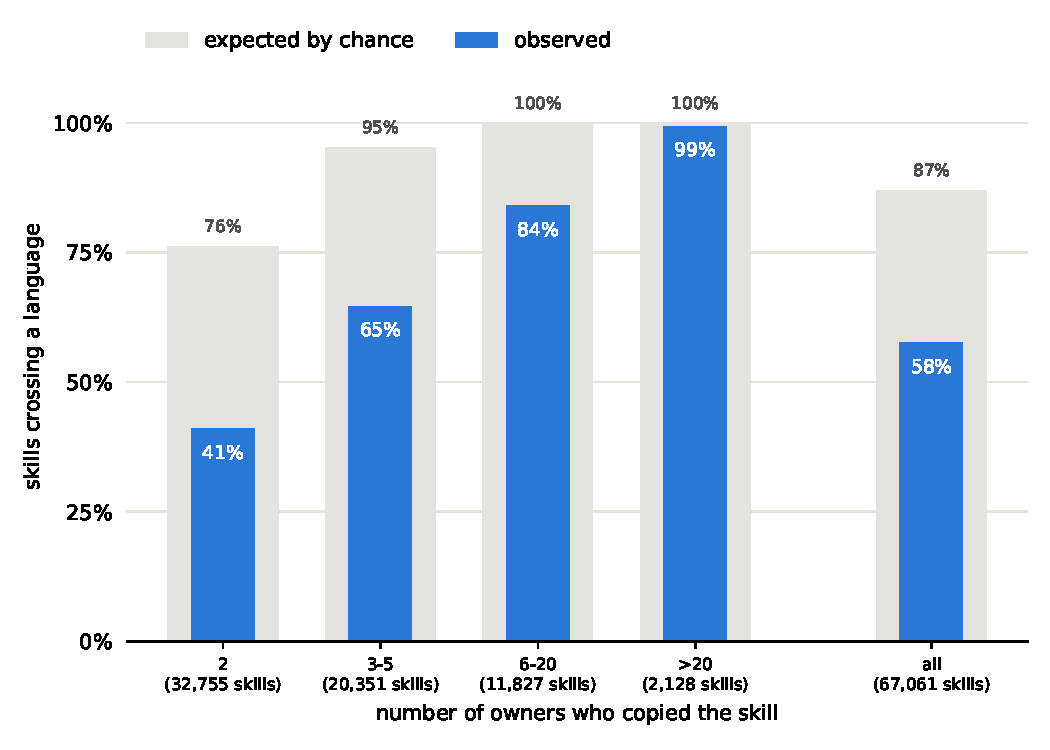
\includegraphics[width=\columnwidth]{rq1_language_crossing.pdf}
\caption{Share of copied skills whose owners use more than one primary language (blue), against the share expected if languages were assigned at random (grey, 1,000 permutations), by number of owners.}
\label{fig:crossing}
\end{figure}

The reuse of a skill often crosses language boundaries, but far less often than it would in a language-agnostic ecosystem. Indeed, 57.6\% of copied skills are used in more than one primary language. In comparison, our permutation baseline, which simulates a language-agnostic ecosystem, expects 87.0\% (Fig.~\ref{fig:crossing}). To check that this gap is not due to chance, we compute a one-sided $p$-value from the shuffles. None of the 1,000 shuffles produced a crossing rate as low as the observed one, so this siloing is very unlikely to be a random effect ($p \le 0.001$).

This difference between reality and the shuffled baseline is not the same for every skill: it depends on how widely a skill has been copied. Skills shared by only two owners cross languages in 41.0\% of cases, against 76.2\% in the shuffled baseline, a 35-point gap (Fig.~\ref{fig:crossing}). The gap narrows as the number of owners grows, and skills with more than 20 owners almost all cross (99.4\%), although with that many owners crossing is almost certain even in the shuffled baseline (100\%). Siloing is therefore strongest among skills with few adopters, while widely copied skills reach most languages.

\begin{figure}[t]
\centering
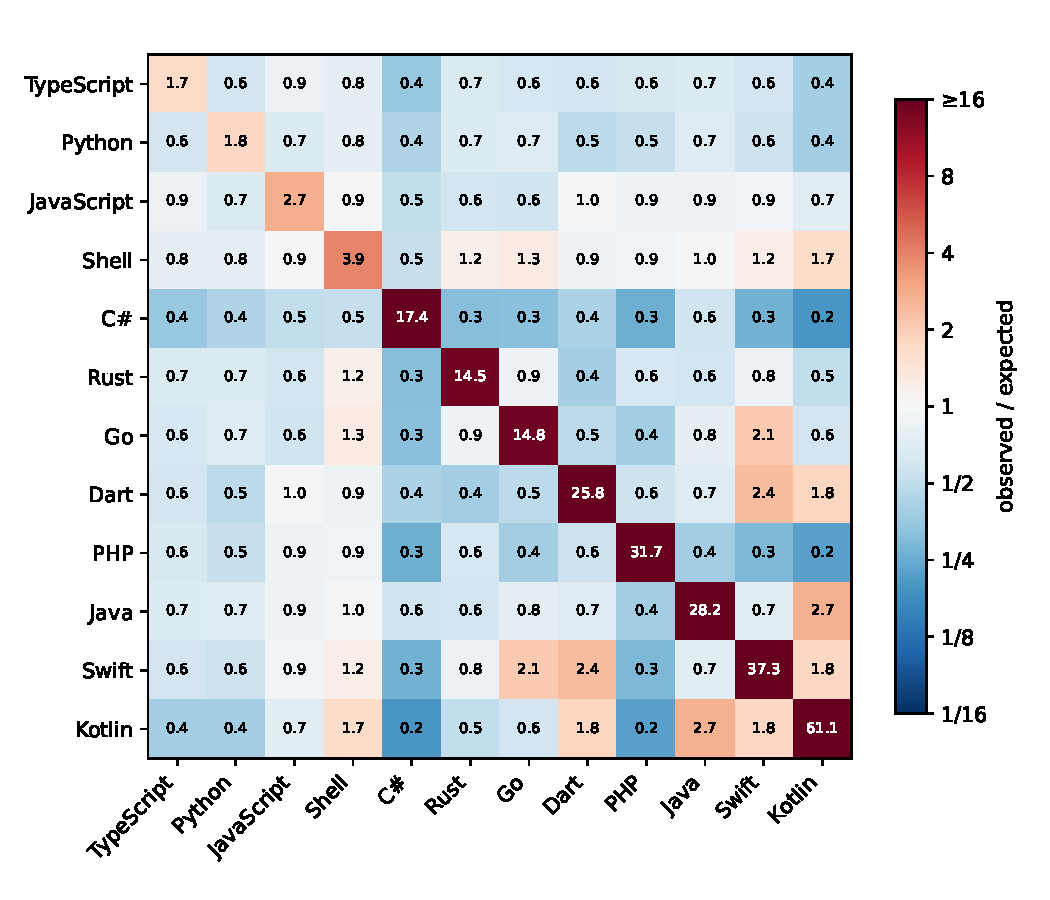
\includegraphics[width=0.85\columnwidth]{rq1_language_heatmap.pdf}
\caption{Skill co-adoption between the 12 largest languages, as the ratio of observed to expected owner pairs (red: more sharing than chance, blue: less).}
\label{fig:heatmap}
\end{figure}

While Fig.~\ref{fig:crossing} measures how much siloing there is overall, the co-adoption matrix in Fig.~\ref{fig:heatmap} shows where it happens. Each diagonal cell tests one language on its own: a value above 1 means its owners share skills with owners of the same language more often than they would in a language-agnostic ecosystem. All 12 diagonal values are above 1, so the siloing in Fig.~\ref{fig:crossing} is not caused by a single community but holds for every language. The effect is strongest for smaller languages: Kotlin (61.1), Swift (37.3), PHP (31.7) and Java (28.2). TypeScript and Python show low ratios (1.7 and 1.8) only because they make up two thirds of all adoptions and thus define the baseline. Ultimately, Off the diagonal, most of the strongest ties link languages that share a runtime (e.g., Java--Kotlin, which both run on the JVM) and mobile development languages (Swift--Dart, Kotlin--Dart, Kotlin--Swift). This essentially indicates that skills cross language boundaries mainly within a shared technical ecosystem, which suggests that silos follow ecosystems as much as languages.

These results also add to previous research on code reuse. Decan et al.~\cite{decan2019empirical} showed that package ecosystems form separate networks for each language, and we observe the same separation for skills, even though skills, unlike packages, are not bound to a language runtime. Bogart et al.~\cite{bogart2021breaking} found that the differences between ecosystems come mainly from community norms rather than technical constraints. Our results point the same way: the \texttt{SKILL.md} format does not prevent cross-language reuse, yet skills remain siloed like other dependencies.

\subsection{RQ2: What Makes a Skill Universal?}

\begin{table}[t]
\caption{Universal vs.\ siloed skills matched on number of owners. Shares in \%, Cliff's $\delta > 0$ means higher for universal skills.}
\label{tab:rq2}
\centering
\begin{tabular}{lrrr}
\toprule
Characteristic & Siloed & Universal & $\delta$ \\
\midrule
Has code block & 63.0 & 49.6 & $-0.13$ \\
\quad code in Shell & 49.0 & 35.3 & \\
\quad code in Python & 11.0 & 6.4 & \\
Has scripts & 17.7 & 8.9 & $-0.09$ \\
Valid front matter & 95.3 & 97.8 & $0.03$ \\
Has reference files & 35.9 & 36.2 & $0.00^{\dagger}$ \\
Text length (chars, mean) & 10,652 & 9,254 & $-0.01^{\dagger}$ \\
\midrule
\multicolumn{4}{l}{\textit{Topics} ($\chi^2 = 306$, $p < 10^{-57}$, Cram\'er's $V = 0.15$)} \\
plan / user / tasks & 13.6 & 19.6 & \\
design / ui / react & 10.0 & 14.7 & \\
data / analysis / database & 13.2 & 9.4 & \\
none (no English word) & 3.8 & 1.4 & \\
\bottomrule
\multicolumn{4}{l}{\footnotesize $^{\dagger}$ not significant after Bonferroni correction.}
\end{tabular}
\end{table}

We compare universal and siloed skills copied by the same number of owners, and find that they look almost the same (Table~\ref{tab:rq2}). Siloed skills include code examples more often (63.0\% vs.\ 49.6\%) and come with script files about twice as often (17.7\% vs.\ 8.9\%). Three of these five differences are statistically significant according to Mann--Whitney $U$ tests with a Bonferroni correction, but all are negligible in size ($|\delta| < 0.147$). This implies that after picking a skill at random from each group, one could hardly tell which group it came from. Siloed skills also more often include Shell (49.0\% vs.\ 35.3\%) and Python (11.0\% vs.\ 6.4\%) code. This is consistent with Gao et al.~\cite{gao2026registry}, who found that when developers adapt a copied skill, they mainly change the parts tied to their own project. Code thus seems to be what ties a skill to its stack, but its effect is too weak to explain the siloing observed in RQ1.

What skills are about differs a bit more than how they are built (Table~\ref{tab:rq2}). The topics of universal and siloed skills are significantly different, but the difference remains small (Cram\'er's $V = 0.15$). Universal skills are more often about work that does not depend on the stack, such as planning tasks (19.6\% vs.\ 13.6\%) and UI design (14.7\% vs.\ 10.0\%), while siloed skills are more often about data and databases (13.2\% vs.\ 9.4\%). Siloed skills are also almost three times as likely to have no English words in their name and description (3.8\% vs.\ 1.4\%), which may point to a second kind of silo, based on human rather than programming language.

The results above show that neither the structure (Table~\ref{tab:rq2}, top) nor the topic (Table~\ref{tab:rq2}, bottom) of a skill differs much between universal and siloed skills, so a skill's content explains only a small part of the siloing observed in RQ1. Combined with the fact that nothing in the \texttt{SKILL.md} format prevents a skill from being used in another language, this suggests that skills stay within a language mainly because of how they circulate between developers, not because of what they contain. For the MSR 2027 Mining Challenge, this means that a language-agnostic format, like the one \texttt{SKILL.md} provides, is not enough to create a language-agnostic ecosystem, and that studies of skill reuse in GitSkills should account for the language of the adopting projects.

\section{Threats to Validity}
\textbf{Construct validity.} We only count exact copies, so a skill that was slightly edited (e.g., a changed path or command) counts as a different skill. If developers adapt skills when moving them to another language, our method misses these cases and may overestimate siloing.

\textbf{Internal validity.} Several thresholds are our own choices: aggregators (more than 100 skills), copied skills (at least two owners) and universal skills (at least three languages). Other values could change the results, and testing them is left for future work.

\section{Conclusion}
This paper studies whether agent skills cross programming language boundaries in the GitSkills dataset. For RQ1, we show that skills often cross languages, but far less often than in a language-agnostic ecosystem: 57.6\% of copied skills reach more than one language, against 87.0\% in our baseline. This siloing is not limited to one community, since every language keeps skills within itself, and the ties that do exist mostly follow shared runtimes and platforms. For RQ2, we find that a skill's content explains little of this siloing: universal and siloed skills have almost the same structure and only slightly different topics. Skills therefore reproduce the language silos known from package ecosystems~\cite{decan2019empirical}, even though, unlike packages, nothing technical forces them to. As Bogart et al.~\cite{bogart2021breaking} observed for package communities, the boundary seems to come from how developers share rather than from the artifacts themselves.

Future work could test this explanation in two ways: (1) use commit history to follow how skills spread between language communities over time, which would show directly how developers share them, and (2) detect near-duplicate copies, to include skills that were adapted when moving to another language and that our exact-match approach misses..
% No preamble here: no \documentclass, \usepackage or \begin{document}.

\begin{abstract}
Agent skills are \texttt{SKILL.md} files written in natural language, so unlike code libraries, which are tied to one language's package ecosystem, they could in principle be reused in any project. Using the GitSkills dataset (3.8 million \texttt{SKILL.md} files in 282,200 GitHub repositories), we find that exact copies of skills often cross programming languages, but far less than in a baseline where language plays no role (57.6\% vs.\ 87.0\%). Those cross-language ties mostly follow shared runtimes and platforms. Since skills that cross languages and skills that do not look almost the same, agent skills seem to reproduce the language silos of package ecosystems for social rather than technical reasons.
\end{abstract}

\section{Introduction}
Traditional software dependencies are tied to a specific programming language and its package ecosystem~\cite{decan2019empirical}. JavaScript libraries are distributed through npm, for example, while Python libraries use PyPI, with each language maintaining its own independent ecosystem. Because these dependencies rely on compilers, specific runtimes, and build toolchains, reuse across language boundaries normally requires wrappers, bindings, or some level of reimplementation. AI coding agents introduce a different possibility through natural-language artifacts, most notably \texttt{SKILL.md} files, which encode workflows, conventions, and recurring developer instructions. Unlike executable code libraries, these artifacts are not bound to a package manager and could therefore be reused across repositories with completely different technology stacks without extra manual effort.

Writing a skill in natural language does not automatically make it portable, however. In practice, a skill can still include language-specific scripts, rely on tools tied to a particular stack, or simply circulate within a single language community, even though nothing in the format itself forces skills to stay siloed. As a result, it remains an open question whether developers are building a unified, language-agnostic skill ecosystem or recreating the same fragmented silos seen in traditional software dependencies.

In this paper, we empirically investigate whether agent skills spread across programming language boundaries using the July 2026 GitSkills dataset~\cite{destefanis2027gitskills}. The dataset collects 3,797,117 \texttt{SKILL.md} files (1,877,981 distinct) across 282,200 public GitHub repositories, linking exact copies by content hash and pairing them with file contents and repository metadata, including each repository's primary programming language. Our goal is to determine whether verbatim skill copying crosses primary programming languages at rates consistent with a language-agnostic ecosystem, and to identify the structural and functional characteristics that distinguish skills that are adopted across multiple language projects from those that are confined to a single language.

Our results actually indicate that verbatim skill copying is only partially independent of programming language. Of the 67,061 skills copied by at least two distinct eligible owners, 57.6\% are adopted across more than one language, compared to 87.0\% in the language-agnostic ecosystem simulated by our baseline. Cross-language adoption is therefore common, yet substantially less frequent than it would be in a language-agnostic ecosystem, pointing to persistent language siloing. Among skills copied by the same number of owners, those adopted across three or more languages also differ from single-language skills, as they are less likely to contain code or scripts and are more frequently associated with language-independent topics such as planning, task management, and UI design. Still, these differences are limited in magnitude, suggesting that a skill's internal structure and topic only explain part of the language concentration we observe.

\section{Background and Related Work}

\subsection{Background}

An agent skill is a folder that contains a \texttt{SKILL.md} file with some YAML front matter (a name and its description) and a Markdown body of natural-language instructions along with optional scripts or some additional reference files~\cite{agentskills_spec,destefanis2027gitskills}. Introduced by Anthropic in October 2025 as an open specification, the format relies on runtime selection (using a probabilistic approach). More specifically, an AI coding agent reads all available skill descriptions added by the agent user and decides at runtime whether to load and use a skill for a given task or not given the current context~\cite{destefanis2027gitskills}. Since those skills do not have a central package manager, developers reuse them mainly by copying folders across repositories no matter the main technology stack of the project~\cite{destefanis2027gitskills}. To identify each repository's technology stack, GitHub actually uses \emph{Linguist}, which is a library that inspects repository files to assign it a primary language in its metadata and classify it as programming, markup, data, or prose. This information that is made available in the GitSkills dataset is fundamental to our research here.

Our analysis relies on four standard statistical and text-mining methods:
\begin{itemize}
    \item \textbf{Permutation testing:} Builds a chance baseline (null distribution) by repeatedly shuffling labels at random, testing how far an observed result departs from chance without parametric assumptions.
    \item \textbf{TF-IDF and NMF:} Term Frequency-Inverse Document Frequency (TF-IDF) converts text into vectors that weight terms frequent in a document but rare across the corpus; Non-negative Matrix Factorization (NMF) decomposes that matrix into interpretable topics.
    \item \textbf{Mann-Whitney U and Cliff's delta:} The Mann-Whitney U test compares two independent groups without assuming normality, while Cliff's delta measures the effect size in $[-1, 1]$ by quantifying how often values in one group exceed those in the other.
    \item \textbf{Chi-square and Cram\'er's V:} Pearson's chi-square test checks whether two categorical variables are associated, and Cram\'er's V scales the strength of that association to $[0, 1]$.
\end{itemize}


\subsection{Related Work}

Before AI coding agents became widespread, empirical work on software reuse focused mainly on artifacts that are directly tied to specific language ecosystems. Studies of package managers showed how dependency networks grow inside separate, language-bound registries such as npm, PyPI, and RubyGems~\cite{decan2019empirical}. Those silos are not only technical as comparing 18 open-source ecosystems, Bogart et al.~\cite{bogart2021breaking} actually showed that language communities also tend to build distinct norms and maintenance practices around their dependencies. Even outside package managers, informal copying reflects ecosystem boundaries. Lopes et al.~\cite{lopes2017dejavu} analyzed 4.5 million GitHub projects and found that 70\% of files are duplicates, with duplication rates varying widely by language (from 94\% in JavaScript to 40\% in Java).

With the arrival of coding agents, reuse studies have expanded to natural-language artifacts such as \texttt{SKILL.md} files among many new techniques for defining reusable artifacts, which are no longer bound to a single runtime. Early work shows that direct copying is still how most reuse happens. More precisely, in GitSkills dataset studied here, 50.5\% of public \texttt{SKILL.md} files are verbatim copies~\cite{destefanis2027gitskills}, and Gao et al.~\cite{gao2026registry} found that skills pulled from community registries into repositories are mostly one-time copies, with later edits focusing on project-specific bindings. At the artifact level, Zhang et al.~\cite{zhang2026keeps} audited 138K \texttt{SKILL.md} files and highlighted that specification and routing-metadata defects frequently limit reuse.

Prior work therefore establishes two things: traditional code reuse was shaped by both technical and community silos, and agent skills are widely copied yet often tied to local project setups. Still, none of these studies test whether natural-language skills actually cross programming-language boundaries or remain concentrated within single-language ecosystems, which is the gap we address here.

\section{Methodology}\label{sec:methodology}

\subsection{Research Questions}
In this study, we address two research questions:
\begin{description}[\IEEEsetlabelwidth{RQ2:}]
    \item[RQ1:] \textit{Ecosystem Silos vs. Universal Flow.} To what extent does the verbatim copying of agent skills bypass traditional programming language boundaries?
    \item[RQ2:] \textit{Anatomy of a Universal Skill.} What structural and functional characteristics distinguish skills adopted across many diverse primary languages from strictly siloed skills?
\end{description}

\subsection{Data Collection and Cleaning}
We use the July 2026 release of the GitSkills dataset~\cite{destefanis2027gitskills}, accessed via its official Hugging Face Parquet mirror (archived on Zenodo, DOI: 10.5281/zenodo.21875637). From it, we extract the \texttt{artifacts} table (3,797,117 \texttt{SKILL.md} files across 1,877,981 unique content hashes) and the \texttt{repos} table (282,200 repositories), keeping file hashes, representative skill contents, and repository metadata.

We clean the data in three stages. First, we filter for repositories whose primary language actually reflects project adoption. Using GitHub Linguist v9.6.0 (the release current at mining time), we keep only repositories with a programming language as their primary language (230,558), excluding markup, data, prose, and undetected languages. We also drop forks (3 repositories) and aggregators holding more than 100 distinct skills (2,829 repositories, just 1.0\% of repositories, yet 54.3\% of all \texttt{SKILL.md} files), since registries, mirrors, and marketplaces do not represent real project use and would bias our insights. This leaves 228,037 eligible repositories.

Second, we identify exact copies using each file's Git blob hash (\texttt{file\_sha}) and store one adoption record per unique skill--repository pair (with \texttt{n\_paths} counting duplicate paths within the same repo). Dropping 1,647,626 single-owner skills leaves 230,355 copied skills (found under at least two distinct owners) and 1,382,321 adoption records overall. We pull structural metadata from each skill's deduplicated representative row, and restrict our language analysis to the 67,061 copied skills adopted by at least two distinct eligible owners. This structural metadata includes each skill's text length, whether its front matter is valid, and whether its folder contains scripts or reference files, as recorded by GitSkills (\texttt{has\_scripts}, \texttt{has\_references}); skills with missing values are excluded from the corresponding comparison.

Third, we extract two content features from each copied skill's representative file. For code blocks, we parse Markdown code fences (\texttt{\`{}\`{}\`{}}) and map their tags to programming languages using Linguist aliases and groups (e.g., mapping \texttt{ts} and \texttt{TSX} to TypeScript). For functional purpose, we combine each skill's \texttt{name} and \texttt{description}, vectorize the text with TF-IDF (removing English stop words, keeping alphabetic tokens of length $\ge 2$ with \texttt{min\_df} $= 20$ and \texttt{max\_df} $= 0.5$), and apply 12-topic NMF (\texttt{nndsvd} initialization, fixed seed). Each skill receives its top-weighted topic (named after its three top terms, which we use to interpret what the topic is about), or \texttt{none} when all topic weights are zero (e.g., non-English or missing text).

\subsection{Analysis and Statistical Methods}
\textbf{RQ1 (Cross-Language Reuse).} Across these skills, we aggregate adoptions at the owner level so that one user copying a skill across many repositories counts only once. Each owner is assigned the most frequent primary language among their eligible repositories holding that skill. We label a skill \emph{cross-language} if its adopting owners span multiple primary languages, and \emph{siloed} otherwise. To account for adoption scale, we group skills into four owner-count tiers: 2, 3--5, 6--20, and $>20$ owners.

Because TypeScript and Python dominate GitHub, some cross-language overlap happens by chance. To separate it from real cross-language flow, we run a 1,000-iteration permutation baseline (fixed seed): in each iteration, we shuffle the primary language labels across skill--owner rows and recompute the overall and per-tier crossing rates. Their mean is the expected rate in a language-agnostic ecosystem (grey bars in Fig.~\ref{fig:crossing}), and the share of shuffles at or below the observed rate gives one-sided $p$-values.

To see which languages actually share skills, we build a co-adoption matrix for the 12 largest languages. For each skill with $k_s$ eligible owners, every pair of distinct owners contributes a language pair weighted by $1/(k_s - 1)$ so popular skills do not dominate. We then divide observed counts by the counts expected under random owner pairing, i.e., in a language-agnostic ecosystem ($>1$ means more sharing than in such an ecosystem).

\textbf{RQ2 (Universal vs. Siloed Skills).} Focusing on skills with at least three eligible owners, we compare \emph{universal skills} ($\ge 3$ primary languages; 14,186 skills) against \emph{siloed skills} (all owners in one language, as in RQ1; 9,104 skills), leaving out two-language skills to keep a clear contrast between the groups. Because popular skills naturally have more chances to span multiple languages, we match both groups on exact owner count by randomly subsampling to the smaller group's size at each count, leaving 6,678 matched pairs (5.1 owners on average).

We compare the matched groups across five structural features (body length, valid YAML front matter, bundled reference files, bundled scripts, and programming-language code blocks) using two-sided Mann--Whitney $U$ tests, Cliff's $\delta$ for effect size, and Bonferroni correction across the five tests, and we also break down code-block shares by individual language. We also test whether topic distributions (the 12 NMF topics plus \texttt{none}) differ between universal and siloed skills using a chi-square test and Cram\'er's $V$.

\subsection{Replication Package}
All notebooks, Linguist language mappings, cleaned CSV datasets and figures are publicly available at \url{https://github.com/Sebastian-Espin/LOG6307E-MSR-2027-mining-challenge}.


\section{Results and Discussion}\label{sec:results}
\subsection{RQ1: Do Copied Skills Cross Language Boundaries?}

\begin{figure}[t]
\centering
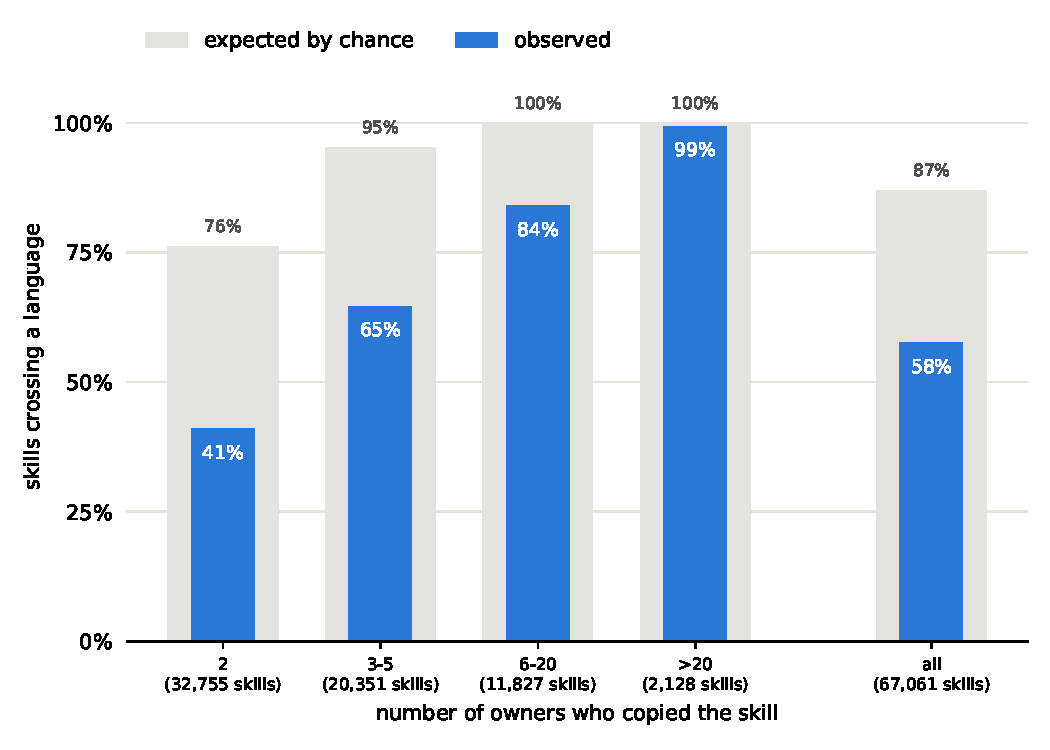
\includegraphics[width=\columnwidth]{rq1_language_crossing.pdf}
\caption{Share of copied skills whose owners use more than one primary language (blue), against the share expected if languages were assigned at random (grey, 1,000 permutations), by number of owners.}
\label{fig:crossing}
\end{figure}

The reuse of a skill often crosses language boundaries, but far less often than it would in a language-agnostic ecosystem. Indeed, 57.6\% of copied skills are used in more than one primary language. In comparison, our permutation baseline, which simulates a language-agnostic ecosystem, expects 87.0\% (Fig.~\ref{fig:crossing}). To check that this gap is not due to chance, we compute a one-sided $p$-value from the shuffles. None of the 1,000 shuffles produced a crossing rate as low as the observed one, so this siloing is very unlikely to be a random effect ($p \le 0.001$).

This difference between reality and the shuffled baseline is not the same for every skill: it depends on how widely a skill has been copied. Skills shared by only two owners cross languages in 41.0\% of cases, against 76.2\% in the shuffled baseline, a 35-point gap (Fig.~\ref{fig:crossing}). The gap narrows as the number of owners grows, and skills with more than 20 owners almost all cross (99.4\%), although with that many owners crossing is almost certain even in the shuffled baseline (100\%). Siloing is therefore strongest among skills with few adopters, while widely copied skills reach most languages.

\begin{figure}[t]
\centering
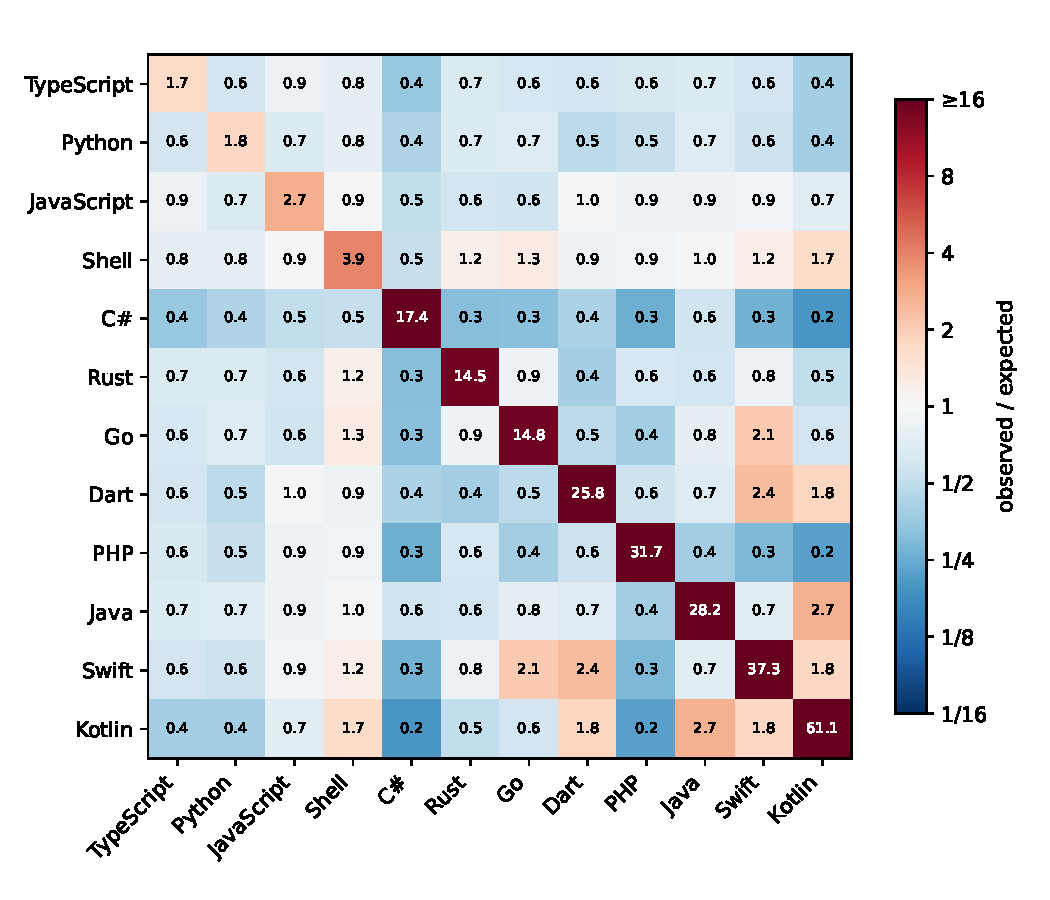
\includegraphics[width=0.85\columnwidth]{rq1_language_heatmap.pdf}
\caption{Skill co-adoption between the 12 largest languages, as the ratio of observed to expected owner pairs (red: more sharing than chance, blue: less).}
\label{fig:heatmap}
\end{figure}

While Fig.~\ref{fig:crossing} measures how much siloing there is overall, the co-adoption matrix in Fig.~\ref{fig:heatmap} shows where it happens. Each diagonal cell tests one language on its own: a value above 1 means its owners share skills with owners of the same language more often than they would in a language-agnostic ecosystem. All 12 diagonal values are above 1, so the siloing in Fig.~\ref{fig:crossing} is not caused by a single community but holds for every language. The effect is strongest for smaller languages: Kotlin (61.1), Swift (37.3), PHP (31.7) and Java (28.2). TypeScript and Python show low ratios (1.7 and 1.8) only because they make up two thirds of all adoptions and thus define the baseline. Ultimately, Off the diagonal, most of the strongest ties link languages that share a runtime (e.g., Java--Kotlin, which both run on the JVM) and mobile development languages (Swift--Dart, Kotlin--Dart, Kotlin--Swift). This essentially indicates that skills cross language boundaries mainly within a shared technical ecosystem, which suggests that silos follow ecosystems as much as languages.

These results also add to previous research on code reuse. Decan et al.~\cite{decan2019empirical} showed that package ecosystems form separate networks for each language, and we observe the same separation for skills, even though skills, unlike packages, are not bound to a language runtime. Bogart et al.~\cite{bogart2021breaking} found that the differences between ecosystems come mainly from community norms rather than technical constraints. Our results point the same way: the \texttt{SKILL.md} format does not prevent cross-language reuse, yet skills remain siloed like other dependencies.

\subsection{RQ2: What Makes a Skill Universal?}

\begin{table}[t]
\caption{Universal vs.\ siloed skills matched on number of owners. Shares in \%, Cliff's $\delta > 0$ means higher for universal skills.}
\label{tab:rq2}
\centering
\begin{tabular}{lrrr}
\toprule
Characteristic & Siloed & Universal & $\delta$ \\
\midrule
Has code block & 63.0 & 49.6 & $-0.13$ \\
\quad code in Shell & 49.0 & 35.3 & \\
\quad code in Python & 11.0 & 6.4 & \\
Has scripts & 17.7 & 8.9 & $-0.09$ \\
Valid front matter & 95.3 & 97.8 & $0.03$ \\
Has reference files & 35.9 & 36.2 & $0.00^{\dagger}$ \\
Text length (chars, mean) & 10,652 & 9,254 & $-0.01^{\dagger}$ \\
\midrule
\multicolumn{4}{l}{\textit{Topics} ($\chi^2 = 306$, $p < 10^{-57}$, Cram\'er's $V = 0.15$)} \\
plan / user / tasks & 13.6 & 19.6 & \\
design / ui / react & 10.0 & 14.7 & \\
data / analysis / database & 13.2 & 9.4 & \\
none (no English word) & 3.8 & 1.4 & \\
\bottomrule
\multicolumn{4}{l}{\footnotesize $^{\dagger}$ not significant after Bonferroni correction.}
\end{tabular}
\end{table}

We compare universal and siloed skills copied by the same number of owners, and find that they look almost the same (Table~\ref{tab:rq2}). Siloed skills include code examples more often (63.0\% vs.\ 49.6\%) and come with script files about twice as often (17.7\% vs.\ 8.9\%). Three of these five differences are statistically significant according to Mann--Whitney $U$ tests with a Bonferroni correction, but all are negligible in size ($|\delta| < 0.147$). This implies that after picking a skill at random from each group, one could hardly tell which group it came from. Siloed skills also more often include Shell (49.0\% vs.\ 35.3\%) and Python (11.0\% vs.\ 6.4\%) code. This is consistent with Gao et al.~\cite{gao2026registry}, who found that when developers adapt a copied skill, they mainly change the parts tied to their own project. Code thus seems to be what ties a skill to its stack, but its effect is too weak to explain the siloing observed in RQ1.

What skills are about differs a bit more than how they are built (Table~\ref{tab:rq2}). The topics of universal and siloed skills are significantly different, but the difference remains small (Cram\'er's $V = 0.15$). Universal skills are more often about work that does not depend on the stack, such as planning tasks (19.6\% vs.\ 13.6\%) and UI design (14.7\% vs.\ 10.0\%), while siloed skills are more often about data and databases (13.2\% vs.\ 9.4\%). Siloed skills are also almost three times as likely to have no English words in their name and description (3.8\% vs.\ 1.4\%), which may point to a second kind of silo, based on human rather than programming language.

The results above show that neither the structure (Table~\ref{tab:rq2}, top) nor the topic (Table~\ref{tab:rq2}, bottom) of a skill differs much between universal and siloed skills, so a skill's content explains only a small part of the siloing observed in RQ1. Combined with the fact that nothing in the \texttt{SKILL.md} format prevents a skill from being used in another language, this suggests that skills stay within a language mainly because of how they circulate between developers, not because of what they contain. For the MSR 2027 Mining Challenge, this means that a language-agnostic format, like the one \texttt{SKILL.md} provides, is not enough to create a language-agnostic ecosystem, and that studies of skill reuse in GitSkills should account for the language of the adopting projects.

\section{Threats to Validity}
\textbf{Construct validity.} We only count exact copies, so a skill that was slightly edited (e.g., a changed path or command) counts as a different skill. If developers adapt skills when moving them to another language, our method misses these cases and may overestimate siloing.

\textbf{Internal validity.} Several thresholds are our own choices: aggregators (more than 100 skills), copied skills (at least two owners) and universal skills (at least three languages). Other values could change the results, and testing them is left for future work.

\section{Conclusion}
This paper studies whether agent skills cross programming language boundaries in the GitSkills dataset. For RQ1, we show that skills often cross languages, but far less often than in a language-agnostic ecosystem: 57.6\% of copied skills reach more than one language, against 87.0\% in our baseline. This siloing is not limited to one community, since every language keeps skills within itself, and the ties that do exist mostly follow shared runtimes and platforms. For RQ2, we find that a skill's content explains little of this siloing: universal and siloed skills have almost the same structure and only slightly different topics. Skills therefore reproduce the language silos known from package ecosystems~\cite{decan2019empirical}, even though, unlike packages, nothing technical forces them to. As Bogart et al.~\cite{bogart2021breaking} observed for package communities, the boundary seems to come from how developers share rather than from the artifacts themselves.

Future work could test this explanation in two ways: (1) use commit history to follow how skills spread between language communities over time, which would show directly how developers share them, and (2) detect near-duplicate copies, to include skills that were adapted when moving to another language and that our exact-match approach misses..
% No preamble here: no \documentclass, \usepackage or \begin{document}.

\begin{abstract}
Agent skills are \texttt{SKILL.md} files written in natural language, so unlike code libraries, which are tied to one language's package ecosystem, they could in principle be reused in any project. Using the GitSkills dataset (3.8 million \texttt{SKILL.md} files in 282,200 GitHub repositories), we find that exact copies of skills often cross programming languages, but far less than in a baseline where language plays no role (57.6\% vs.\ 87.0\%). Those cross-language ties mostly follow shared runtimes and platforms. Since skills that cross languages and skills that do not look almost the same, agent skills seem to reproduce the language silos of package ecosystems for social rather than technical reasons.
\end{abstract}

\section{Introduction}
Traditional software dependencies are tied to a specific programming language and its package ecosystem~\cite{decan2019empirical}. JavaScript libraries are distributed through npm, for example, while Python libraries use PyPI, with each language maintaining its own independent ecosystem. Because these dependencies rely on compilers, specific runtimes, and build toolchains, reuse across language boundaries normally requires wrappers, bindings, or some level of reimplementation. AI coding agents introduce a different possibility through natural-language artifacts, most notably \texttt{SKILL.md} files, which encode workflows, conventions, and recurring developer instructions. Unlike executable code libraries, these artifacts are not bound to a package manager and could therefore be reused across repositories with completely different technology stacks without extra manual effort.

Writing a skill in natural language does not automatically make it portable, however. In practice, a skill can still include language-specific scripts, rely on tools tied to a particular stack, or simply circulate within a single language community, even though nothing in the format itself forces skills to stay siloed. As a result, it remains an open question whether developers are building a unified, language-agnostic skill ecosystem or recreating the same fragmented silos seen in traditional software dependencies.

In this paper, we empirically investigate whether agent skills spread across programming language boundaries using the July 2026 GitSkills dataset~\cite{destefanis2027gitskills}. The dataset collects 3,797,117 \texttt{SKILL.md} files (1,877,981 distinct) across 282,200 public GitHub repositories, linking exact copies by content hash and pairing them with file contents and repository metadata, including each repository's primary programming language. Our goal is to determine whether verbatim skill copying crosses primary programming languages at rates consistent with a language-agnostic ecosystem, and to identify the structural and functional characteristics that distinguish skills that are adopted across multiple language projects from those that are confined to a single language.

Our results actually indicate that verbatim skill copying is only partially independent of programming language. Of the 67,061 skills copied by at least two distinct eligible owners, 57.6\% are adopted across more than one language, compared to 87.0\% in the language-agnostic ecosystem simulated by our baseline. Cross-language adoption is therefore common, yet substantially less frequent than it would be in a language-agnostic ecosystem, pointing to persistent language siloing. Among skills copied by the same number of owners, those adopted across three or more languages also differ from single-language skills, as they are less likely to contain code or scripts and are more frequently associated with language-independent topics such as planning, task management, and UI design. Still, these differences are limited in magnitude, suggesting that a skill's internal structure and topic only explain part of the language concentration we observe.

\section{Background and Related Work}

\subsection{Background}

An agent skill is a folder that contains a \texttt{SKILL.md} file with some YAML front matter (a name and its description) and a Markdown body of natural-language instructions along with optional scripts or some additional reference files~\cite{agentskills_spec,destefanis2027gitskills}. Introduced by Anthropic in October 2025 as an open specification, the format relies on runtime selection (using a probabilistic approach). More specifically, an AI coding agent reads all available skill descriptions added by the agent user and decides at runtime whether to load and use a skill for a given task or not given the current context~\cite{destefanis2027gitskills}. Since those skills do not have a central package manager, developers reuse them mainly by copying folders across repositories no matter the main technology stack of the project~\cite{destefanis2027gitskills}. To identify each repository's technology stack, GitHub actually uses \emph{Linguist}, which is a library that inspects repository files to assign it a primary language in its metadata and classify it as programming, markup, data, or prose. This information that is made available in the GitSkills dataset is fundamental to our research here.

Our analysis relies on four standard statistical and text-mining methods:
\begin{itemize}
    \item \textbf{Permutation testing:} Builds a chance baseline (null distribution) by repeatedly shuffling labels at random, testing how far an observed result departs from chance without parametric assumptions.
    \item \textbf{TF-IDF and NMF:} Term Frequency-Inverse Document Frequency (TF-IDF) converts text into vectors that weight terms frequent in a document but rare across the corpus; Non-negative Matrix Factorization (NMF) decomposes that matrix into interpretable topics.
    \item \textbf{Mann-Whitney U and Cliff's delta:} The Mann-Whitney U test compares two independent groups without assuming normality, while Cliff's delta measures the effect size in $[-1, 1]$ by quantifying how often values in one group exceed those in the other.
    \item \textbf{Chi-square and Cram\'er's V:} Pearson's chi-square test checks whether two categorical variables are associated, and Cram\'er's V scales the strength of that association to $[0, 1]$.
\end{itemize}


\subsection{Related Work}

Before AI coding agents became widespread, empirical work on software reuse focused mainly on artifacts that are directly tied to specific language ecosystems. Studies of package managers showed how dependency networks grow inside separate, language-bound registries such as npm, PyPI, and RubyGems~\cite{decan2019empirical}. Those silos are not only technical as comparing 18 open-source ecosystems, Bogart et al.~\cite{bogart2021breaking} actually showed that language communities also tend to build distinct norms and maintenance practices around their dependencies. Even outside package managers, informal copying reflects ecosystem boundaries. Lopes et al.~\cite{lopes2017dejavu} analyzed 4.5 million GitHub projects and found that 70\% of files are duplicates, with duplication rates varying widely by language (from 94\% in JavaScript to 40\% in Java).

With the arrival of coding agents, reuse studies have expanded to natural-language artifacts such as \texttt{SKILL.md} files among many new techniques for defining reusable artifacts, which are no longer bound to a single runtime. Early work shows that direct copying is still how most reuse happens. More precisely, in GitSkills dataset studied here, 50.5\% of public \texttt{SKILL.md} files are verbatim copies~\cite{destefanis2027gitskills}, and Gao et al.~\cite{gao2026registry} found that skills pulled from community registries into repositories are mostly one-time copies, with later edits focusing on project-specific bindings. At the artifact level, Zhang et al.~\cite{zhang2026keeps} audited 138K \texttt{SKILL.md} files and highlighted that specification and routing-metadata defects frequently limit reuse.

Prior work therefore establishes two things: traditional code reuse was shaped by both technical and community silos, and agent skills are widely copied yet often tied to local project setups. Still, none of these studies test whether natural-language skills actually cross programming-language boundaries or remain concentrated within single-language ecosystems, which is the gap we address here.

\section{Methodology}\label{sec:methodology}

\subsection{Research Questions}
In this study, we address two research questions:
\begin{description}[\IEEEsetlabelwidth{RQ2:}]
    \item[RQ1:] \textit{Ecosystem Silos vs. Universal Flow.} To what extent does the verbatim copying of agent skills bypass traditional programming language boundaries?
    \item[RQ2:] \textit{Anatomy of a Universal Skill.} What structural and functional characteristics distinguish skills adopted across many diverse primary languages from strictly siloed skills?
\end{description}

\subsection{Data Collection and Cleaning}
We use the July 2026 release of the GitSkills dataset~\cite{destefanis2027gitskills}, accessed via its official Hugging Face Parquet mirror (archived on Zenodo, DOI: 10.5281/zenodo.21875637). From it, we extract the \texttt{artifacts} table (3,797,117 \texttt{SKILL.md} files across 1,877,981 unique content hashes) and the \texttt{repos} table (282,200 repositories), keeping file hashes, representative skill contents, and repository metadata.

We clean the data in three stages. First, we filter for repositories whose primary language actually reflects project adoption. Using GitHub Linguist v9.6.0 (the release current at mining time), we keep only repositories with a programming language as their primary language (230,558), excluding markup, data, prose, and undetected languages. We also drop forks (3 repositories) and aggregators holding more than 100 distinct skills (2,829 repositories, just 1.0\% of repositories, yet 54.3\% of all \texttt{SKILL.md} files), since registries, mirrors, and marketplaces do not represent real project use and would bias our insights. This leaves 228,037 eligible repositories.

Second, we identify exact copies using each file's Git blob hash (\texttt{file\_sha}) and store one adoption record per unique skill--repository pair (with \texttt{n\_paths} counting duplicate paths within the same repo). Dropping 1,647,626 single-owner skills leaves 230,355 copied skills (found under at least two distinct owners) and 1,382,321 adoption records overall. We pull structural metadata from each skill's deduplicated representative row, and restrict our language analysis to the 67,061 copied skills adopted by at least two distinct eligible owners. This structural metadata includes each skill's text length, whether its front matter is valid, and whether its folder contains scripts or reference files, as recorded by GitSkills (\texttt{has\_scripts}, \texttt{has\_references}); skills with missing values are excluded from the corresponding comparison.

Third, we extract two content features from each copied skill's representative file. For code blocks, we parse Markdown code fences (\texttt{\`{}\`{}\`{}}) and map their tags to programming languages using Linguist aliases and groups (e.g., mapping \texttt{ts} and \texttt{TSX} to TypeScript). For functional purpose, we combine each skill's \texttt{name} and \texttt{description}, vectorize the text with TF-IDF (removing English stop words, keeping alphabetic tokens of length $\ge 2$ with \texttt{min\_df} $= 20$ and \texttt{max\_df} $= 0.5$), and apply 12-topic NMF (\texttt{nndsvd} initialization, fixed seed). Each skill receives its top-weighted topic (named after its three top terms, which we use to interpret what the topic is about), or \texttt{none} when all topic weights are zero (e.g., non-English or missing text).

\subsection{Analysis and Statistical Methods}
\textbf{RQ1 (Cross-Language Reuse).} Across these skills, we aggregate adoptions at the owner level so that one user copying a skill across many repositories counts only once. Each owner is assigned the most frequent primary language among their eligible repositories holding that skill. We label a skill \emph{cross-language} if its adopting owners span multiple primary languages, and \emph{siloed} otherwise. To account for adoption scale, we group skills into four owner-count tiers: 2, 3--5, 6--20, and $>20$ owners.

Because TypeScript and Python dominate GitHub, some cross-language overlap happens by chance. To separate it from real cross-language flow, we run a 1,000-iteration permutation baseline (fixed seed): in each iteration, we shuffle the primary language labels across skill--owner rows and recompute the overall and per-tier crossing rates. Their mean is the expected rate in a language-agnostic ecosystem (grey bars in Fig.~\ref{fig:crossing}), and the share of shuffles at or below the observed rate gives one-sided $p$-values.

To see which languages actually share skills, we build a co-adoption matrix for the 12 largest languages. For each skill with $k_s$ eligible owners, every pair of distinct owners contributes a language pair weighted by $1/(k_s - 1)$ so popular skills do not dominate. We then divide observed counts by the counts expected under random owner pairing, i.e., in a language-agnostic ecosystem ($>1$ means more sharing than in such an ecosystem).

\textbf{RQ2 (Universal vs. Siloed Skills).} Focusing on skills with at least three eligible owners, we compare \emph{universal skills} ($\ge 3$ primary languages; 14,186 skills) against \emph{siloed skills} (all owners in one language, as in RQ1; 9,104 skills), leaving out two-language skills to keep a clear contrast between the groups. Because popular skills naturally have more chances to span multiple languages, we match both groups on exact owner count by randomly subsampling to the smaller group's size at each count, leaving 6,678 matched pairs (5.1 owners on average).

We compare the matched groups across five structural features (body length, valid YAML front matter, bundled reference files, bundled scripts, and programming-language code blocks) using two-sided Mann--Whitney $U$ tests, Cliff's $\delta$ for effect size, and Bonferroni correction across the five tests, and we also break down code-block shares by individual language. We also test whether topic distributions (the 12 NMF topics plus \texttt{none}) differ between universal and siloed skills using a chi-square test and Cram\'er's $V$.

\subsection{Replication Package}
All notebooks, Linguist language mappings, cleaned CSV datasets and figures are publicly available at \url{https://github.com/Sebastian-Espin/LOG6307E-MSR-2027-mining-challenge}.


\section{Results and Discussion}\label{sec:results}
\subsection{RQ1: Do Copied Skills Cross Language Boundaries?}

\begin{figure}[t]
\centering
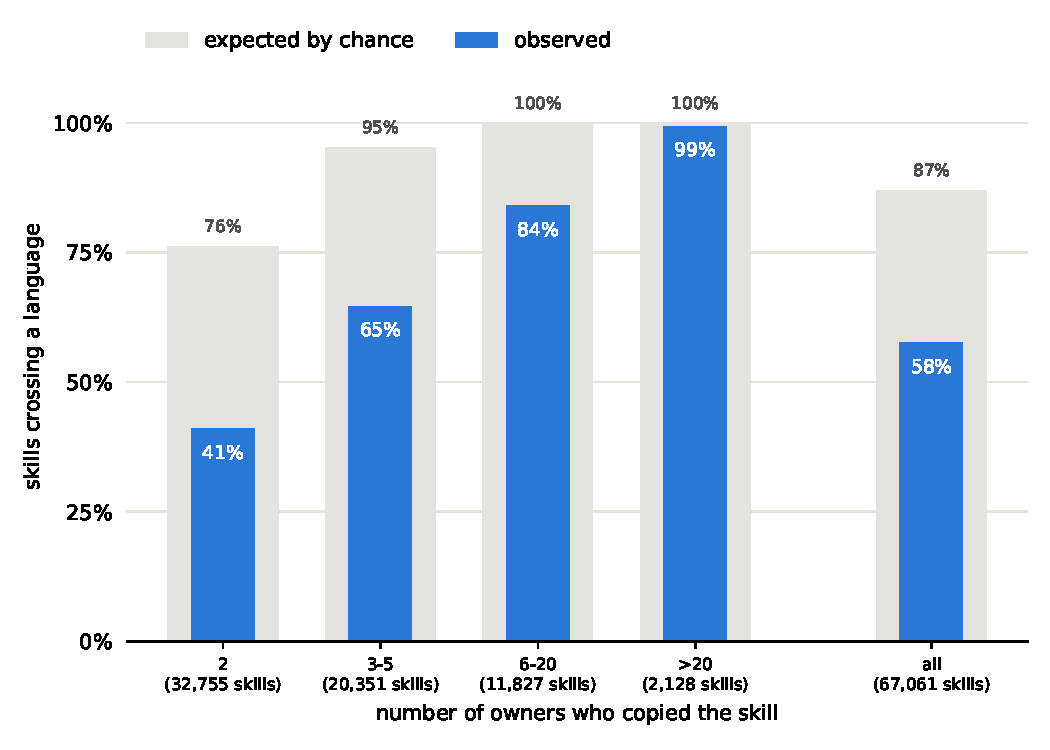
\includegraphics[width=\columnwidth]{rq1_language_crossing.pdf}
\caption{Share of copied skills whose owners use more than one primary language (blue), against the share expected if languages were assigned at random (grey, 1,000 permutations), by number of owners.}
\label{fig:crossing}
\end{figure}

The reuse of a skill often crosses language boundaries, but far less often than it would in a language-agnostic ecosystem. Indeed, 57.6\% of copied skills are used in more than one primary language. In comparison, our permutation baseline, which simulates a language-agnostic ecosystem, expects 87.0\% (Fig.~\ref{fig:crossing}). To check that this gap is not due to chance, we compute a one-sided $p$-value from the shuffles. None of the 1,000 shuffles produced a crossing rate as low as the observed one, so this siloing is very unlikely to be a random effect ($p \le 0.001$).

This difference between reality and the shuffled baseline is not the same for every skill: it depends on how widely a skill has been copied. Skills shared by only two owners cross languages in 41.0\% of cases, against 76.2\% in the shuffled baseline, a 35-point gap (Fig.~\ref{fig:crossing}). The gap narrows as the number of owners grows, and skills with more than 20 owners almost all cross (99.4\%), although with that many owners crossing is almost certain even in the shuffled baseline (100\%). Siloing is therefore strongest among skills with few adopters, while widely copied skills reach most languages.

\begin{figure}[t]
\centering
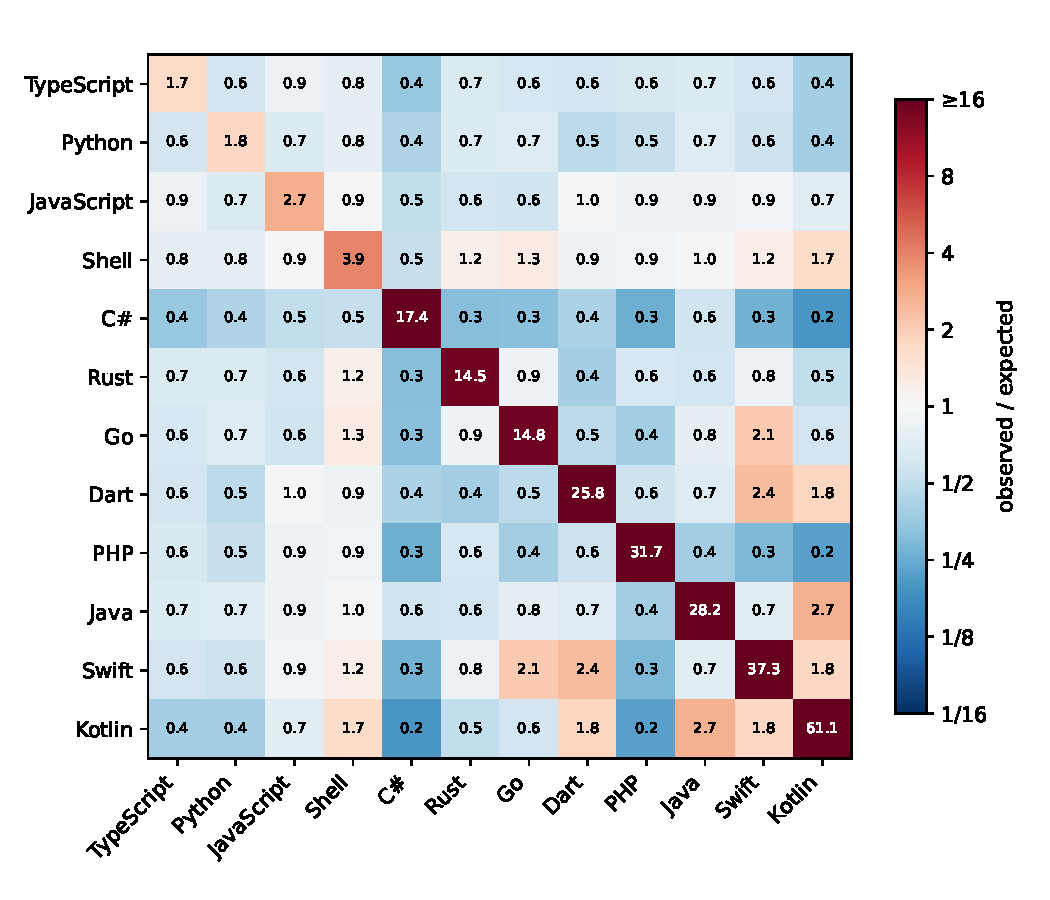
\includegraphics[width=0.85\columnwidth]{rq1_language_heatmap.pdf}
\caption{Skill co-adoption between the 12 largest languages, as the ratio of observed to expected owner pairs (red: more sharing than chance, blue: less).}
\label{fig:heatmap}
\end{figure}

While Fig.~\ref{fig:crossing} measures how much siloing there is overall, the co-adoption matrix in Fig.~\ref{fig:heatmap} shows where it happens. Each diagonal cell tests one language on its own: a value above 1 means its owners share skills with owners of the same language more often than they would in a language-agnostic ecosystem. All 12 diagonal values are above 1, so the siloing in Fig.~\ref{fig:crossing} is not caused by a single community but holds for every language. The effect is strongest for smaller languages: Kotlin (61.1), Swift (37.3), PHP (31.7) and Java (28.2). TypeScript and Python show low ratios (1.7 and 1.8) only because they make up two thirds of all adoptions and thus define the baseline. Ultimately, Off the diagonal, most of the strongest ties link languages that share a runtime (e.g., Java--Kotlin, which both run on the JVM) and mobile development languages (Swift--Dart, Kotlin--Dart, Kotlin--Swift). This essentially indicates that skills cross language boundaries mainly within a shared technical ecosystem, which suggests that silos follow ecosystems as much as languages.

These results also add to previous research on code reuse. Decan et al.~\cite{decan2019empirical} showed that package ecosystems form separate networks for each language, and we observe the same separation for skills, even though skills, unlike packages, are not bound to a language runtime. Bogart et al.~\cite{bogart2021breaking} found that the differences between ecosystems come mainly from community norms rather than technical constraints. Our results point the same way: the \texttt{SKILL.md} format does not prevent cross-language reuse, yet skills remain siloed like other dependencies.

\subsection{RQ2: What Makes a Skill Universal?}

\begin{table}[t]
\caption{Universal vs.\ siloed skills matched on number of owners. Shares in \%, Cliff's $\delta > 0$ means higher for universal skills.}
\label{tab:rq2}
\centering
\begin{tabular}{lrrr}
\toprule
Characteristic & Siloed & Universal & $\delta$ \\
\midrule
Has code block & 63.0 & 49.6 & $-0.13$ \\
\quad code in Shell & 49.0 & 35.3 & \\
\quad code in Python & 11.0 & 6.4 & \\
Has scripts & 17.7 & 8.9 & $-0.09$ \\
Valid front matter & 95.3 & 97.8 & $0.03$ \\
Has reference files & 35.9 & 36.2 & $0.00^{\dagger}$ \\
Text length (chars, mean) & 10,652 & 9,254 & $-0.01^{\dagger}$ \\
\midrule
\multicolumn{4}{l}{\textit{Topics} ($\chi^2 = 306$, $p < 10^{-57}$, Cram\'er's $V = 0.15$)} \\
plan / user / tasks & 13.6 & 19.6 & \\
design / ui / react & 10.0 & 14.7 & \\
data / analysis / database & 13.2 & 9.4 & \\
none (no English word) & 3.8 & 1.4 & \\
\bottomrule
\multicolumn{4}{l}{\footnotesize $^{\dagger}$ not significant after Bonferroni correction.}
\end{tabular}
\end{table}

We compare universal and siloed skills copied by the same number of owners, and find that they look almost the same (Table~\ref{tab:rq2}). Siloed skills include code examples more often (63.0\% vs.\ 49.6\%) and come with script files about twice as often (17.7\% vs.\ 8.9\%). Three of these five differences are statistically significant according to Mann--Whitney $U$ tests with a Bonferroni correction, but all are negligible in size ($|\delta| < 0.147$). This implies that after picking a skill at random from each group, one could hardly tell which group it came from. Siloed skills also more often include Shell (49.0\% vs.\ 35.3\%) and Python (11.0\% vs.\ 6.4\%) code. This is consistent with Gao et al.~\cite{gao2026registry}, who found that when developers adapt a copied skill, they mainly change the parts tied to their own project. Code thus seems to be what ties a skill to its stack, but its effect is too weak to explain the siloing observed in RQ1.

What skills are about differs a bit more than how they are built (Table~\ref{tab:rq2}). The topics of universal and siloed skills are significantly different, but the difference remains small (Cram\'er's $V = 0.15$). Universal skills are more often about work that does not depend on the stack, such as planning tasks (19.6\% vs.\ 13.6\%) and UI design (14.7\% vs.\ 10.0\%), while siloed skills are more often about data and databases (13.2\% vs.\ 9.4\%). Siloed skills are also almost three times as likely to have no English words in their name and description (3.8\% vs.\ 1.4\%), which may point to a second kind of silo, based on human rather than programming language.

The results above show that neither the structure (Table~\ref{tab:rq2}, top) nor the topic (Table~\ref{tab:rq2}, bottom) of a skill differs much between universal and siloed skills, so a skill's content explains only a small part of the siloing observed in RQ1. Combined with the fact that nothing in the \texttt{SKILL.md} format prevents a skill from being used in another language, this suggests that skills stay within a language mainly because of how they circulate between developers, not because of what they contain. For the MSR 2027 Mining Challenge, this means that a language-agnostic format, like the one \texttt{SKILL.md} provides, is not enough to create a language-agnostic ecosystem, and that studies of skill reuse in GitSkills should account for the language of the adopting projects.

\section{Threats to Validity}
\textbf{Construct validity.} We only count exact copies, so a skill that was slightly edited (e.g., a changed path or command) counts as a different skill. If developers adapt skills when moving them to another language, our method misses these cases and may overestimate siloing.

\textbf{Internal validity.} Several thresholds are our own choices: aggregators (more than 100 skills), copied skills (at least two owners) and universal skills (at least three languages). Other values could change the results, and testing them is left for future work.

\section{Conclusion}
This paper studies whether agent skills cross programming language boundaries in the GitSkills dataset. For RQ1, we show that skills often cross languages, but far less often than in a language-agnostic ecosystem: 57.6\% of copied skills reach more than one language, against 87.0\% in our baseline. This siloing is not limited to one community, since every language keeps skills within itself, and the ties that do exist mostly follow shared runtimes and platforms. For RQ2, we find that a skill's content explains little of this siloing: universal and siloed skills have almost the same structure and only slightly different topics. Skills therefore reproduce the language silos known from package ecosystems~\cite{decan2019empirical}, even though, unlike packages, nothing technical forces them to. As Bogart et al.~\cite{bogart2021breaking} observed for package communities, the boundary seems to come from how developers share rather than from the artifacts themselves.

Future work could test this explanation in two ways: (1) use commit history to follow how skills spread between language communities over time, which would show directly how developers share them, and (2) detect near-duplicate copies, to include skills that were adapted when moving to another language and that our exact-match approach misses.

% ---------------------------------------------------------------
\bibliographystyle{IEEEtran}
\bibliography{references}

\end{document}
